\section{Architecture} \label{sec:architecture}
\subsection{Overview} \label{sec:architecture:overview}
In simple terms, a BF machine consists of an array of memory-cells, together with a pointer pointing to one of these cells. The pointer can move along the array while modifying its contents one step at a time. Figure \ref{fig:simplerepresentation} illustrates an example intermediate state of such a system. Consider the BF program ``\texttt{>>>>>+.}'', applied to the initial conditions shown in the example. The pointer would take 5 steps to the right, landing on cell 9 which contains the number 41. It will then increment and output this value, displaying 42 on the screen (assuming a screen of some sort is used as the output device and it is displaying numbers directly rather than interpreting them as ASCII).

\begin{figure}[H]
  \centering
  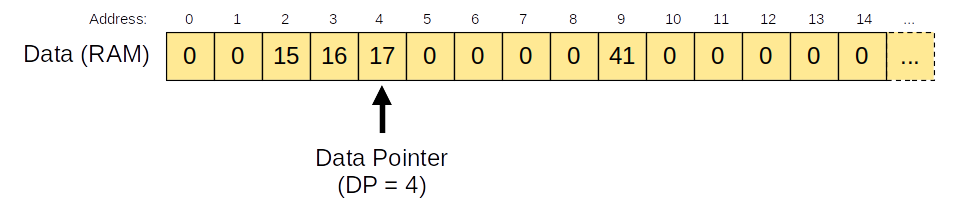
\includegraphics[width=0.9\textwidth]{img/simple_representation}
  \caption{Example state of a BF machine.}
  \label{fig:simplerepresentation}
\end{figure}


The processor consists of three basic building blocks: registers, memory and a control unit. The ALU is missing from this list because the only operations that it needs to perform are addition and subtraction of the value 1, which can be done directly at the register-level when using up/down binary counters like the 74LS193 integrated circuit. The program (a sequence of BF instructions) is stored into Read Only Memory (ROM), whereas the data is stored in Random Access Memory (RAM). Instructions (4-bits) are fed from ROM into the control unit (CU) together with five flags (K, A, V, S and Z) that encode the state of the machine. Depending on the state and current instruction, the CU sets the appropriate control signals for each of the modules in order for the system to perform the next computation. Figure \ref{fig:architecture} shows how each of the modules is communicating with other modules. In the sections below, each of these connections will be clarified further. The actual implementation on the logic/hardware level is described in Section \ref{sec:implementation}.

\begin{figure}[H]
  \centering
  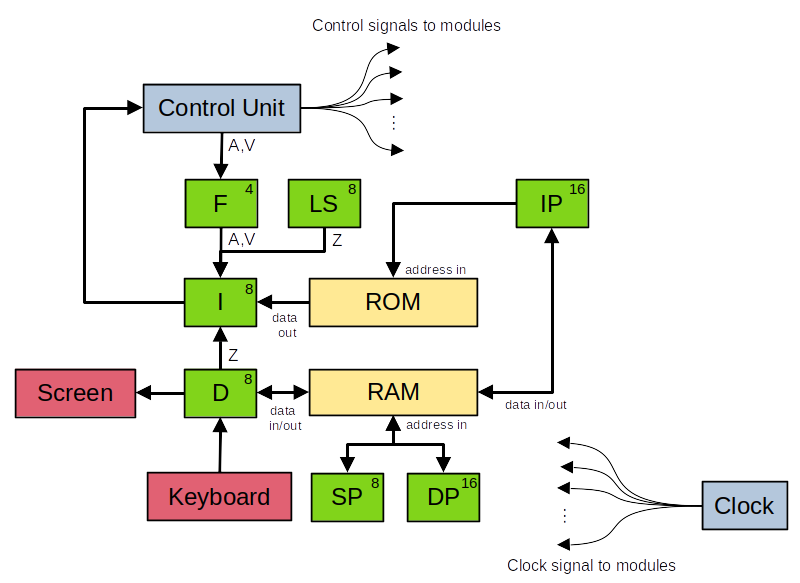
\includegraphics[width=0.9\textwidth]{img/bfcpu_architecture}
  \caption{Connections between modules in the BF processor.}
  \label{fig:architecture}
\end{figure}


\subsection{Data Pointer Register (DP)} \label{sec:architecture:dp}
The data-pointer corresponds to the pointer as specified in the BF-language. It points to some value in memory beyond the stack ($\ge$ 0x0100, see \ref{sec:architecture:sp}) and can be either incremented (moved right) or decremented (moved left) using the \texttt{>} and \texttt{<} instructions. Whenever the value pointed to by DP is modified by \texttt{+} or \texttt{-}, it is loaded into the D-register (see \ref{sec:architecture:d}), where it can be modified before being stored back into RAM.

\subsubsection*{Inputs}
The DP should be able to increment and decrement (corresponding to the \texttt{<} and \texttt{>} commands), and should be able to be enabled/disabled because of its connection to the address bus of the RAM (the Stack Pointer (SP, see \ref{sec:architecture:sp}, is also connected to this bus). While all other modules have the ability to be reset, the DP is the only register that can be reset (to 0x0100) at runtime. This is necessary during boot, when all the datacells need to be initialized to 0 (see \ref{seq:sequences:nonbf}).

\begin{itemize}
\itemsep0em 
\item EN - Enable - Assert the stored 16-bit value onto the address bus.
\item U - Up - Increment the stored value.
\item D - Down - Decrement the stored value.
\item R - Reset - Reset the value to 0x0100, the start of the datasection of RAM.
\end{itemize}

\subsubsection*{Outputs}
\begin{itemize}
\itemsep0em   
\item DP\_OUT - 16 bits, asserted onto the address bus when enabled (EN high).
\end{itemize}

\subsection{Data Register (D)} \label{sec:architecture:d}
The data register holds a representation of the value currently pointed to by the DP and can be incremented and decremented (corresponding to \texttt{+} and \texttt{-}). This register provides the Z flag to signify that its current value is 0. Among other things, this flag can be used to determine whether or not to enter a loop.

\subsubsection*{Inputs}
\begin{itemize}
\itemsep0em   
\item D\_IN - 8 bits - Data inputs, connected to the databus.
\item EN - Enable - Assert the stored value onto the databus.
\item LD - Load - Load data from the bus into D.
\item U - Up - Increment the stored value.
\item D - Down - Decrement the stored value.
\end{itemize}

\subsubsection*{Outputs}
\begin{itemize}
\itemsep0em 
\item D\_OUT - 8 bits - Data outputs, connected to the databus.
\item SET\_Z - Set Zero Flag - High when the register stores a zero, connected to FB.
\end{itemize}


\subsection{Instruction Pointer Register (IP)} \label{sec:architecture:ip}
The IP Register stores the instruction pointer (16-bits), which keeps track of the instruction that is currently being executed. It points to a certain address in ROM (which stores the program) and is usually incremented after each instruction has finished executing, in order to move to the next instruction. However, when the processor encounters the \texttt{[}-instruction (and a loop is entered), its value is stored in RAM at the location pointed to by the stack pointer (SP, see \ref{sec:architecture:sp}). When the matching \texttt{]}-instruction is encountered, this value can be loaded back into the IP in order to jump back to the start of the loop if needed.

\subsubsection*{Inputs}
\begin{itemize}
\itemsep0em 
\item IP\_IN - 16 bits - Data inputs, connected to the databus.
\item EN - Enable - Assert the stored value onto the databus.
\item LD - Load - Load data from the bus into IP.
\item U - Up -Increment the stored value. 
\end{itemize}

\subsubsection*{Outputs}
\begin{itemize}
\itemsep0em 
\item IP\_OUT - 16 bits - Data outputs, connected to the databus and the address inputs of program-ROM;
\end{itemize}


\subsection{Stack Pointer Register (SP)} \label{sec:architecture:sp}
The stack is the first part of RAM (addresses 0x0000 - 0x00ff) and is reserved to keep track of addresses in ROM that might need to be jumped to when flow encounters a loop-end instruction (\texttt{]}). The stack-pointer (SP) points to an address in this space; it is incremented whenever a new jump-address is pushed to the stack and decremented whenever an address is popped off the stack. In this implementation, the SP is an 8-bit value, which means that at most 256 different values can be stored onto the stack before it the SP overflows (wraps around back to 0) and starts overwriting previous values. This would happen if a BF program was loaded that has more than 256 nested \texttt{[]}-pairs. Although possible, it is very unlikely to happen for the simple programs we intend to run.

\subsubsection*{Inputs}
\begin{itemize}
\itemsep0em 
\item EN - Enable - Assert the stack-pointer onto the address-bus.
\item U - Up - Increment the stack-pointer.
\item D - Down - Decrement the stack-pointer.
\end{itemize}

\subsubsection*{Outputs}
\begin{itemize}
\itemsep0em 
\item SP\_OUT - 8 bits - connected to the address bus of RAM.
\end{itemize}

\subsection{Loop Skip Register (LS)} \label{sec:architecture:ls}
The Loop Skip (LS) register is a counter that indicates whether or not we're in the process of skipping a loop. In BF, a loop (\texttt{[}) is only entered when the value currently pointed to is nonzero. In the case that it is zero, execution resumes beyond its matching loop-end instruction (\texttt{]}). When it is determined that a loop must be skipped (based on the Z-flag of the D-register), the LS register is incremented from 0 to 1 and the S-flag is set. Subsequent instructions are then skipped until either another (nested) loop-start or a closing loop-end is encountered. On the former, the LS is incremented again while on the latter the LS is decremented. This has the effect that the LS becomes 0 again after the \texttt{]} that matches the original \texttt{[} which led to the skip. Normal execution occurs as soon as LS has become 0 again and the S-flag is reset back to 0.

\subsubsection*{Inputs}
\begin{itemize}
  \itemsep0em
\item U - Up - Increment the stored value.
\item D - Down - Decrement the stored value.
\end{itemize}

\subsubsection*{Outputs}
\begin{itemize}
\itemsep0em 
\item SET\_S - Skip flag - set when it value is nonzero, connected to FB.
\end{itemize}

\subsection{Flag Registers (FA and FB)} \label{sec:architecture:flags}
The first flag register (FA) holds two flag values A and V which are used to indicate that either the address or value respectively has changed during one of the previous instructions. For instance, if D was incremented, the V-flag is set to indicate a change of the \emph{value} being pointed to (the value in RAM is now outdated). For a more detailed description of the function and application of these flags, refer to Section \ref{sec:sequences:+-} and \ref{sec:sequences:<>}. On the zeroth cycle of every instruction, these flags are latched into the FB register together with the Z and S flags (set by the D and LS registers) for a total of 4 flags. The previously mentioned K-flag is specific to interactions with the IO-module and will be discussed in Sections \ref{sec:sequences:output} and \ref{sec:sequences:input}.

\subsubsection*{Inputs}
\begin{itemize}
\itemsep0em 
\item SET\_A - Set the address-change-flag.
\item SET\_V - Set the value-change-flag.
\item LD(FA) - Load A and V into FA.
\item LD(FB) - Load A, V (previously buffered in FA), Z and S (from D and LS) into FB. 
\end{itemize}

\subsubsection*{Outputs}
\begin{itemize}
\itemsep0em 
\item F\_OUT - 4 bits - connected to the instruction decoder inside the Control Unit.
\end{itemize}


\subsection{Instruction Register (I)} \label{sec:architecture:i}
The instruction register I buffers the current instruction pointed to by the IP. The instruction is loaded from program ROM into I at the start of every new instruction, right after IP has been incremented. Its outputs are used as the instruction-part that go into the decoder of the CU (see Figure \ref{fig:decoder} in Section \ref{sec:sequences}).


\subsubsection*{Inputs}
\begin{itemize}
\itemsep0em 
\item LD(I) - Load the instruction pointed to by IP
\end{itemize}

\subsubsection*{Outputs}
\begin{itemize}
\itemsep0em 
\item I\_OUT - 4 bits - connected to the instruction decoder inside the Control Unit.
\end{itemize}


\subsection{Register Driver} \label{sec:architecture:registerdriver}
Rather than having a separate signal for each of the INC/DEC-inputs of each register (e.g.~ INC\_D, INC\_LS, etc), a driver module was designed (see \ref{sec:implementation:registerdriver}) to drive register modules that support modification of their contents. In addition to a universal INC/DEC signal, three Register Select (RS) bits are used to index the target-register. This approach has two advantages:
\begin{enumerate}
\item It decreases the amount of control signals needed;
\item The logic needed to drive the counting registers (74LS193) only needs to be implemented once.
\end{enumerate}

The driver module accepts 5 control signals: 3 register-select signals (RS0 through RS2), INC and DEC. Using 3 register-select signals, up to 8 ($2^3$) registers can be selected, though only 5 need to be driven by the driver. Table \ref{tab:registers} contains an overview of each of the registers and the control signals they support.

\begin{table}[H]
  \centering
  \begin{tabular}{c|c|c|c|c|c|c}
    Register & \#Bits & EN  & LD  & INC  & DEC & RS2$|$RS1$|$RS0 \\ \hline 
    D        & 8      & x   & x   & x    & x   & 0$|$0$|$1 \\
    DP       & 16     & x   &     & x    & x   & 0$|$1$|$0 \\ 
    SP       & 8      & x   &     & x    & x   & 0$|$1$|$1 \\ 
    IP       & 16     & x   & x   & x    &     & 1$|$0$|$0 \\ 
    LS       & 8      &     &     & x    & x   & 1$|$0$|$1 \\ 
    FA       & 4      &     & x   &      &     & not addressable \\ 
    FB       & 4      &     & x   &      &     & not addressable  \\
    I        & 4      &     & x   &      &     & not addressable \\
  \end{tabular}
  \caption{Control signals available on each of the registers. The flag and instruction registers are not connected to the register driver.}
  \label{tab:registers}
\end{table}

\subsubsection*{Inputs}
\begin{itemize}
  \itemsep0em
\item RS0 - Register Select Bit 0
\item RS1 - Register Select Bit 1
\item RS2 - Register Select Bit 2
\item INC - Increment selected register
\item DEC - Decrement selected register
\end{itemize}

\subsubsection*{Outputs}
\begin{itemize}
\itemsep0em 
\item U - 5 bits - Up signals - Connected to the U input of all registers that support the INC operation.
\item D - 5 bits - Down-signals - Connected to the D input of all registers that support the DEC operation.
\end{itemize}


\subsection{Cycle Counter (CC)} \label{sec:architecture:cc}
Almost every BF instruction requires multiple cycles to complete. Therefore, in addition to the instruction and state, a cycle counter is used to determine the control signals that should be sent out.  This cycle counter is a 3-bit counting register (allowing for at most 8 cycles per instruction) that increments on every clock cycle and sends its output to the control unit. Its only control signal is the Cycle Reset (CR) signal which resets the count in order to fetch the next instruction (which happens on cycle 0).

\subsubsection*{Inputs}
\begin{itemize}
\itemsep0em
\item CR - Cycle Reset - Reset the count to 0;
\end{itemize}

\subsubsection*{Outputs}
\begin{itemize}
\itemsep0em
\item CC\_OUT - 3 bits - Current value of the register (0-8).
\end{itemize}

\subsection{Data Memory (RAM)}  \label{sec:architecture:ram}
RAM is divided into two parts: stack and data. The first 256 bytes (0x0000 - 0x00ff) make up the stack and are indexed by the stack pointer (\ref{sec:architecture:sp}). The data (corresponding to the BF tape) is stored at addresses 0x0100 through 0xffff and are indexed by the data pointer (\ref{sec:architecture:dp}). 

\subsubsection*{Inputs}
\begin{itemize}
\itemsep0em 
\item DATA\_IN - 16 bits - Input data, connected to the databus.
\item ADDR\_IN - 16 bits - Address lines, connected to the address bus;
\item OE - Output Enable - Assert the value stored at the current address onto the databus;
\item WE - Write Enable - Write the value on the databus into the current address.
\end{itemize}

\subsubsection*{Outputs}
\begin{itemize}
\itemsep0em 
\item DATA\_OUT - 16 bits - Output data, connected to the databus (same physical lines as DATA\_IN).
\end{itemize}

\subsection{Program Memory (ROM)} \label{sec:architecture:rom}
The actual BF instructions are stored in Read-Only-Memory (ROM) and are addressed by the IP (\ref{sec:architecture:ip}). A 4-bit instruction is stored at the address pointed to by the IP. It is sent to the CU where it is used to determine the set of control signals, together with the flags and cycle counter.

\subsubsection*{Inputs}
\begin{itemize}
\itemsep0em 
\item ADDR\_IN - 16 bits - Address lines, connected to the IP.
\end{itemize}

\subsubsection*{Outputs}
\begin{itemize}
\itemsep0em 
\item INS\_OUT - 4 bits - Instruction data, connected to the CU.
\end{itemize}


\subsection{Screen (SCR)}  \label{sec:architecture:scr}
The output module (which is assumed to be a screen) will be attached to the data bus and will display whatever is on the bus  when enabled using the EN signal. Because the output is handled asynchronously by some peripheral that will, from the perspective of the CPU, be viewed as a black box, it needs a flag to acknowledge a successful data-transfer. This is done through the K-flag, which is set by the peripheral after reading data from the databus (this flag is shared with the input device for a similar purpose). This flag can only be reset by the CU, indicating that the transfer procedure has been completed.
\subsubsection*{Inputs}
\begin{itemize}
\itemsep0em 
\item DATA\_IN - 8 bits - connected to the data bus.
\item EN: Enable - Display the contents of the bus. The format of the output (ASCII, hex, etc) may vary depending on the implementation of the output device.
\item CLR\_K - Clears the K-flag - connected to the CU
\end{itemize}

\subsubsection*{Outputs}
None.

\subsection{Keyboard (KB)} \label{sec:architecture:kb}
The input device to the computer is assumed to be a keyboard of some sort\footnote{At a later stage in the process of building the CPU, a Random Number Generator (RNG) was implemented as a second input device, to support a common Brainf*ck extension, where \texttt{?} is used to generate a random number in the currently active cell.}, that implements a buffer from which some 8-bit value can be requested. The control unit can assert the enable-signal of this device and should then wait until the K-flag is set, indicating that the data is ready to be read from the databus. It is left up to the implementation of the peripheral to decide what to do when there is nothing in the buffer (either wait for user input or return 0). Shared with the output-peripheral, the K\_REC signal is used to indicate that the K-flag has been received and reset, indicating that the data has been transferred and the input-device can yield control of the databus back to the system.

\subsubsection*{Inputs}
\begin{itemize}
\itemsep0em 
\item EN - Enable - Make the contents of the input buffer available on the databus.
\item CLR\_K - Clears the K-flag - connected to the CU.
\end{itemize}

\subsubsection*{Outputs}
\begin{itemize}
\itemsep0em 
\item DATA\_OUT - 8 bits - Output data, connected to the databus.
\end{itemize}



\subsection{Control Unit} \label{sec:architecture:cu}
Each of the aforementioned components/modules has one or more control inputs that determine what happens on the next clock cycle. For example, some register-modules can be told to load a value from their input, increment or decrement the currently stored value, or do nothing at all. It is the Control Unit (CU) that supplies the appropriate control signals to each of the modules before the next clock pulse occurs, depending on the current instruction and state determined by the flags and cycle counter. The implementation details of how this is done in hardware are discussed in Section \ref{sec:implementation}.

\subsubsection*{Inputs}
\begin{itemize}
\itemsep0em
\item CC\_IN - 3 bits - Cycle counter input lines.
\item INS\_IN - 4 bits - Instruction input lines (from program ROM).
\item FLAGS\_IN - 5 bits - Flag input lines (from FB and K).
\end{itemize}

\subsubsection*{Outputs}
\begin{itemize}
\itemsep0em 
\item HLT - Halt Clock
\item RS0 - Register Select, bit 0
\item RS1 - Register Select, bit 1
\item RS2 - Register Select, bit 2
\item INC - Increment selected register
\item DEC - Decrement selected register
\item CLR - Reset DP
\item EN\_SP- Enable SP to address bus \footnote{Note that there is no EN\_DP since this signal is mutually exclusive with EN\_SP; whenever one is set, the other is unset and vice versa.}
\item OE\_RAM - Output Enable RAM
\item WE\_RAM - Write Enable RAM
\item EN\_IN - Enable input (keyboard) to databus
\item EN\_OUT - Enable output device
\item SET\_V - Set V flag in FA
\item SET\_A - Set A flag in FA
\item LD\_FB - Load FB
\item LD\_FA - Load FA
\item EN\_IP - Enable IP
\item EN\_D - Enable D to databus
\item LD\_D - Load D
\item LD\_IP - Load IP
\item CR - Cycle Reset
\item CLR\_K - Clear the K-flag in the IO module
\item ERR - Error Signal
\end{itemize}


